\documentclass[tikz,border=10pt]{standalone}
% Scale: s = 0.011976 cm/px (longest side ~8 cm); y flipped about y_px = 432
\begin{document}
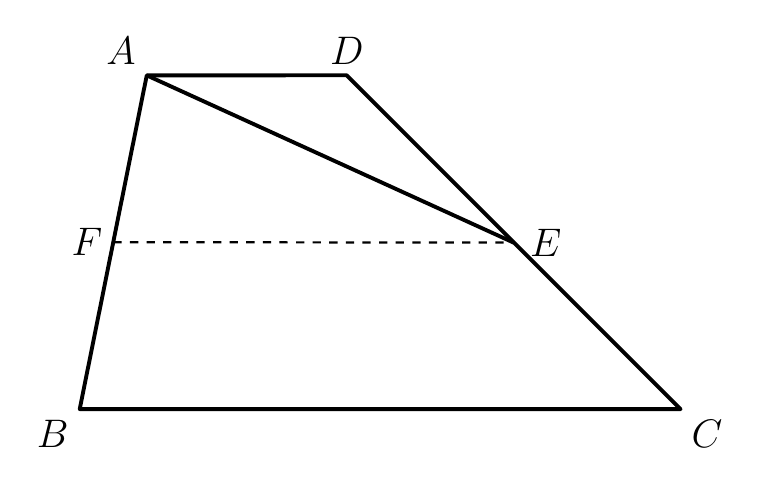
\begin{tikzpicture}[line width=1.4pt, line join=round]
  % Named coordinates (converted from pixels; unchanged)
  \coordinate (A) at (1.4599, 4.2385);
  \coordinate (D) at (4.0000, 4.2396);
  \coordinate (B) at (0.6084, 0);
  \coordinate (C) at (8.2389, 0);
  \coordinate (E) at (6.1181, 2.1151);
  \coordinate (F) at (1.0359, 2.1199);

  % Solid trapezoid edges and diagonal-like segment A-E
  \draw (A) -- (D) -- (C) -- (B) -- cycle;
  \draw (A) -- (E);

  % Dashed segment F-E: lighter stroke, 3pt on / 3pt off dashes
  \draw[line width=0.8pt, dash pattern=on 3pt off 3pt] (F) -- (E);

  % Labels (14 pt font from cap-height metrics)
  \node[above left] at (A) {\fontsize{14}{16.8}\selectfont $A$};
  \node[above] at (D) {\fontsize{14}{16.8}\selectfont $D$};
  \node[below left] at (B) {\fontsize{14}{16.8}\selectfont $B$};
  \node[below right] at (C) {\fontsize{14}{16.8}\selectfont $C$};
  % E: directly right of the vertex, level with it, small 2pt xshift
  \node[right, xshift=2pt] at (E) {\fontsize{14}{16.8}\selectfont $E$};
  \node[left] at (F) {\fontsize{14}{16.8}\selectfont $F$};
\end{tikzpicture}
\end{document}